\documentclass[shownotes,11pt, aspectratio=169]{beamer}

\usepackage{pgfpages}
% These slides also contain speaker notes. You can print just the slides,
% just the notes, or both, depending on the setting below. Comment out the want
% you want.
\setbeameroption{hide notes} % Only slide
%\setbeameroption{show only notes} % Only notes
%\setbeameroption{show notes on second screen=right} % Both

\usepackage{helvet}
\usepackage[default]{Fira Sans}
\usepackage{array}
\usepackage{caption}
%\usepackage[clean]{svg}
\usepackage{tikz}
\usepackage{verbatim}
\setbeamertemplate{note page}{\pagecolor{yellow!5}\insertnote}
\usetikzlibrary{positioning}
\usetikzlibrary{snakes}
\usetikzlibrary{calc}
\usetikzlibrary{arrows}
\usetikzlibrary{decorations.markings}
\usetikzlibrary{shapes.misc}
\usetikzlibrary{matrix,shapes,arrows,fit,tikzmark}
\usepackage{amsmath}
\usepackage{mathpazo}
\usepackage{hyperref}
\usepackage{lipsum}
\usepackage{multimedia}
\usepackage{graphicx}
\usepackage{multirow}
%\usepackage{graphicx}
\usepackage{dcolumn}
\usepackage{bbm}
\usepackage{tfrupee}

%%%%more packages%%%
\usepackage{tabulary}
%\usepackage[usenames,dvipsnames]{pstricks}
%\usepackage[capposition=top]{floatrow}
\usepackage{lineno,hyperref}
\usepackage{epsfig}
\usepackage{graphics}
\usepackage{psfrag}
\usepackage{etoolbox}
\appto\TPTnoteSettings{\footnotesize}
\usepackage{color}
\usepackage{amsfonts}
\usepackage{amsmath}
\usepackage{mathrsfs}
\usepackage{eucal}
\usepackage{amsbsy}
\usepackage{url}
\usepackage{color}
\usepackage{lineno}
\usepackage{amssymb}
%\usepackage{adjustbox}
\newcommand{\overbar}[1]{\mkern 2.5mu\overline{\mkern-2.5mu#1\mkern-2.5mu}\mkern 2.5mu}
\usepackage{booktabs} %%To use toprule, midrule, bottomrule, etc.
\usepackage{rotating} %% To use sidewaystable 
\usepackage{dcolumn}
\usepackage{longtable}
\usepackage{threeparttable}
\usepackage{tabularx}
%%%%

\newcolumntype{d}[0]{D{.}{.}{5}}

\usepackage{changepage}
\usepackage{appendixnumberbeamer}
\newcommand{\beginbackup}{
   \newcounter{framenumbervorappendix}
   \setcounter{framenumbervorappendix}{\value{framenumber}}
   \setbeamertemplate{footline}
   {
     \leavevmode%
     \hline
     box{%
       \begin{beamercolorbox}[wd=\paperwidth,ht=2.25ex,dp=1ex,right]{footlinecolor}%
%         \insertframenumber  \hspace*{2ex} 
       \end{beamercolorbox}}%
     \vskip0pt%
   }
 }
\newcommand{\backupend}{
   \addtocounter{framenumbervorappendix}{-\value{framenumber}}
   \addtocounter{framenumber}{\value{framenumbervorappendix}} 
}


\usepackage{graphicx}
\usepackage[space]{grffile}

% These are my colors -- there are many like them, but these ones are mine.
\definecolor{blue}{RGB}{0,114,178}
\definecolor{red}{RGB}{213,94,0}
\definecolor{yellow}{RGB}{240,228,66}
\definecolor{green}{RGB}{0,158,115}
\definecolor{applegreen}{rgb}{0.55, 0.71, 0.0}
\definecolor{ao(english)}{rgb}{0.0, 0.5, 0.0}

\hypersetup{
  colorlinks=false,
  bookmarks=true,
  linkbordercolor = {white},
  linkcolor = {blue}
}


%% I use a beige off white for my background
\definecolor{MyBackground}{RGB}{255,253,218}

%% Uncomment this if you want to change the background color to something else
\setbeamercolor{background canvas}{bg=MyBackground}

%% Change the bg color to adjust your transition slide background color!
\newenvironment{transitionframe}{
  \setbeamercolor{background canvas}{bg=yellow}
  \begin{frame}}{
    \end{frame}
}

\setbeamercolor{frametitle}{fg=blue}
\setbeamercolor{title}{fg=black}
\setbeamertemplate{footline}[frame number]
\setbeamertemplate{navigation symbols}{} 
\setbeamertemplate{itemize items}{-}
\setbeamercolor{itemize item}{fg=blue}
\setbeamercolor{itemize subitem}{fg=blue}
\setbeamercolor{enumerate item}{fg=blue}
\setbeamercolor{enumerate subitem}{fg=blue}
\setbeamercolor{button}{bg=MyBackground,fg=blue,}



% If you like road maps, rather than having clutter at the top, have a roadmap show up at the end of each section 
% (and after your introduction)
% Uncomment this is if you want the roadmap!
% \AtBeginSection[]
% {
%    \begin{frame}
%        \frametitle{Roadmap of Talk}
%        \tableofcontents[currentsection]
%    \end{frame}
% }
\setbeamercolor{section in toc}{fg=blue}
\setbeamercolor{subsection in toc}{fg=red}
\setbeamersize{text margin left=1em,text margin right=1em} 

\newenvironment{wideitemize}{\itemize\addtolength{\itemsep}{10pt}}{\enditemize}

\title[]{\textcolor{blue}{Macroeconomics: Lecture 6}}
\author[SM]{Sumit Mishra}
\institute[IFMR]{\small{\begin{tabular}{c}
IFMR, Sri City \\
\end{tabular}}}

\date{14 October, 2019}

%\documentclass[10pt]{beamer}
%\input{slideclass.tex}







%----------------------------------------------------------------------------------------
%	TITLE PAGE
%----------------------------------------------------------------------------------------


\begin{document}


\section{Introduction}
\begin{frame}
\titlepage % Print the title page as the first slide
\end{frame}
%\colorlinks=true
%\begin{frame}
%\frametitle{Overview} % Table of contents slide, comment this block out to remove it
%\tableofcontents % Throughout your presentation, if you choose to use \section{} and \subsection{} commands, these will automatically be printed on this slide as an overview of your presentation
%\end{frame}

%----------------------------------------------------------------------------------------
%	PRESENTATION SLIDES
%----------------------------------------------------------------------------------------

%------------------------------------------------
%\section{Preliminaries} 
%\subsection{Introduction}
\begin{frame}
\frametitle{Introduction}
Why growth matters? \\
Data on infant mortality rates:
\begin{itemize}
 \item 20\% in the poorest 1/5 of all countries
  \item 0.4\% in the richest 1/5
   \item In Malawi, more than 70\% of people live on less than \$2/day.
\end{itemize}   
One-fourth of the poorest countries have had
famines during the past 3 decades. \\
Poverty is associated with oppression of women
and minorities.
\end{frame}


\begin{frame}
\frametitle{Income and Poverty in the World}    
 \begin{figure}[ht]
\centering
  \makebox[0.55\linewidth][c]{
  \includegraphics[clip,width=0.8\linewidth]{graphs/poverty_income_pc.png}}
%\caption*{Lemonade Price Is Always Fixed at 0.75c}}
\end{figure}
\end{frame}


\begin{frame}
Fact 1: \textbf{There is enormous variation in per capita income across economies. The poorest countries have per capita incomes that are less than 5 percent of per capita income in the richest countries.}

\vspace{.25in}\noindent Several notes:
\begin{itemize}
	\item Income per capita (or GDP per capita) is not the sole measure of what is good: but it's a useful summary statistic
	\item Income per capita ignores distribution of income within a country
	\item Comparing income per capita across countries is not trivial
	\begin{itemize}
		\item You have to convert between currencies
		\item Countries have different relative prices for goods
		\item What is the ``right'' way to value haircuts, apples, or cars across countries?
	\end{itemize}
\end{itemize}
\end{frame}

\begin{frame}
\frametitle{Rich Countries}
%\linespread{1}
%\begin{tiny}
\makebox[\linewidth][c]{
\begin{tabular}{lccccc}\hline
 & GDP per capita & GDP per worker & LF Part. Rate & Avg. Growth & Years to \\
Country & 2008 & 2008 & 2008 & 1960-2008 &  Double \\ \hline \hline
United States  & \$43,326 & \$84,771 & 0.51 & 1.6 & 43 \\
Japan & 33,735 & 64,778 & 0.52 & 3.4 & 21 \\
France & 31,980 & 69,910 & 0.46 & 2.2 & 30 \\
United Kingdom & 35,345 & 70,008 & 0.51 & 1.9 & 36 \\
Spain & 28,958 & 57,786 & 0.50 & 2.7 & 26 \\ \hline
\end{tabular}}
%\end{tiny}
\end{frame}

\begin{frame}
\frametitle{Poor Countries}
%\linespread{1}
%\begin{small}
\makebox[\linewidth][c]{
\begin{tabular}{lccccc}\hline
 & GDP per capita & GDP per worker & LF Part. Rate & Avg. Growth & Years to \\
Country & 2008 & 2008 & 2008 & 1960-2008 &  Double \\ \hline \hline
China & 6,415 & 10,938 & 0.59 & 5.6 & 13 \\
India & 3,078 & 7,801 & 0.39 & 3.0 & 24 \\
Nigeria & 1,963 & 6,106 & 0.32 & 0.6 & 114 \\
Uganda & 1,122 & 2,604 & 0.43 & 1.3 & 52 \\ \hline
\end{tabular}}
%\end{small}
\end{frame}

\begin{frame}
\frametitle{Growth Miracles}
\begin{tabular}{lccccc}\hline
 & GDP per capita & GDP per worker & LF Part. Rate & Avg. Growth & Years to \\
Country & 2008 & 2008 & 2008 & 1960-2008 &  Double \\ \hline \hline
Hong Kong & 37,834 & 70,940 & 0.53 & 4.3 & 16 \\
Singapore & 49,987 & 92,634 & 0.54 & 4.1 & 17 \\
Taiwan & 29,645 & 62,610 & 0.47 & 5.1 & 14 \\
South Korea & 25,539 & 50,988 & 0.50 & 4.5 & 16 \\ \hline
\end{tabular}
\end{frame}

\begin{frame}
\frametitle{Growth Disasters}
\begin{tabular}{lccccc}\hline
 & GDP per capita & GDP per worker & LF Part. Rate & Avg. Growth & Years to \\
Country & 2008 & 2008 & 2008 & 1960-2008 &  Double \\ \hline \hline
Venezuela & 9,762 & 21,439 & 0.46 & -0.1 & -627 \\
Haiti & 1,403 & 3,164 & 0.44 & -0.4 & -168 \\
Madagascar & 810 & 1,656 & 0.49 & -0.1 & -488 \\
Zimbabwe & 135 & 343 & 0.40 & -1.5 & -47 \\  \hline
\end{tabular}
\end{frame}

\begin{frame}
\frametitle{Distribution of Population by GDP per Worker, 2008}
\begin{center}
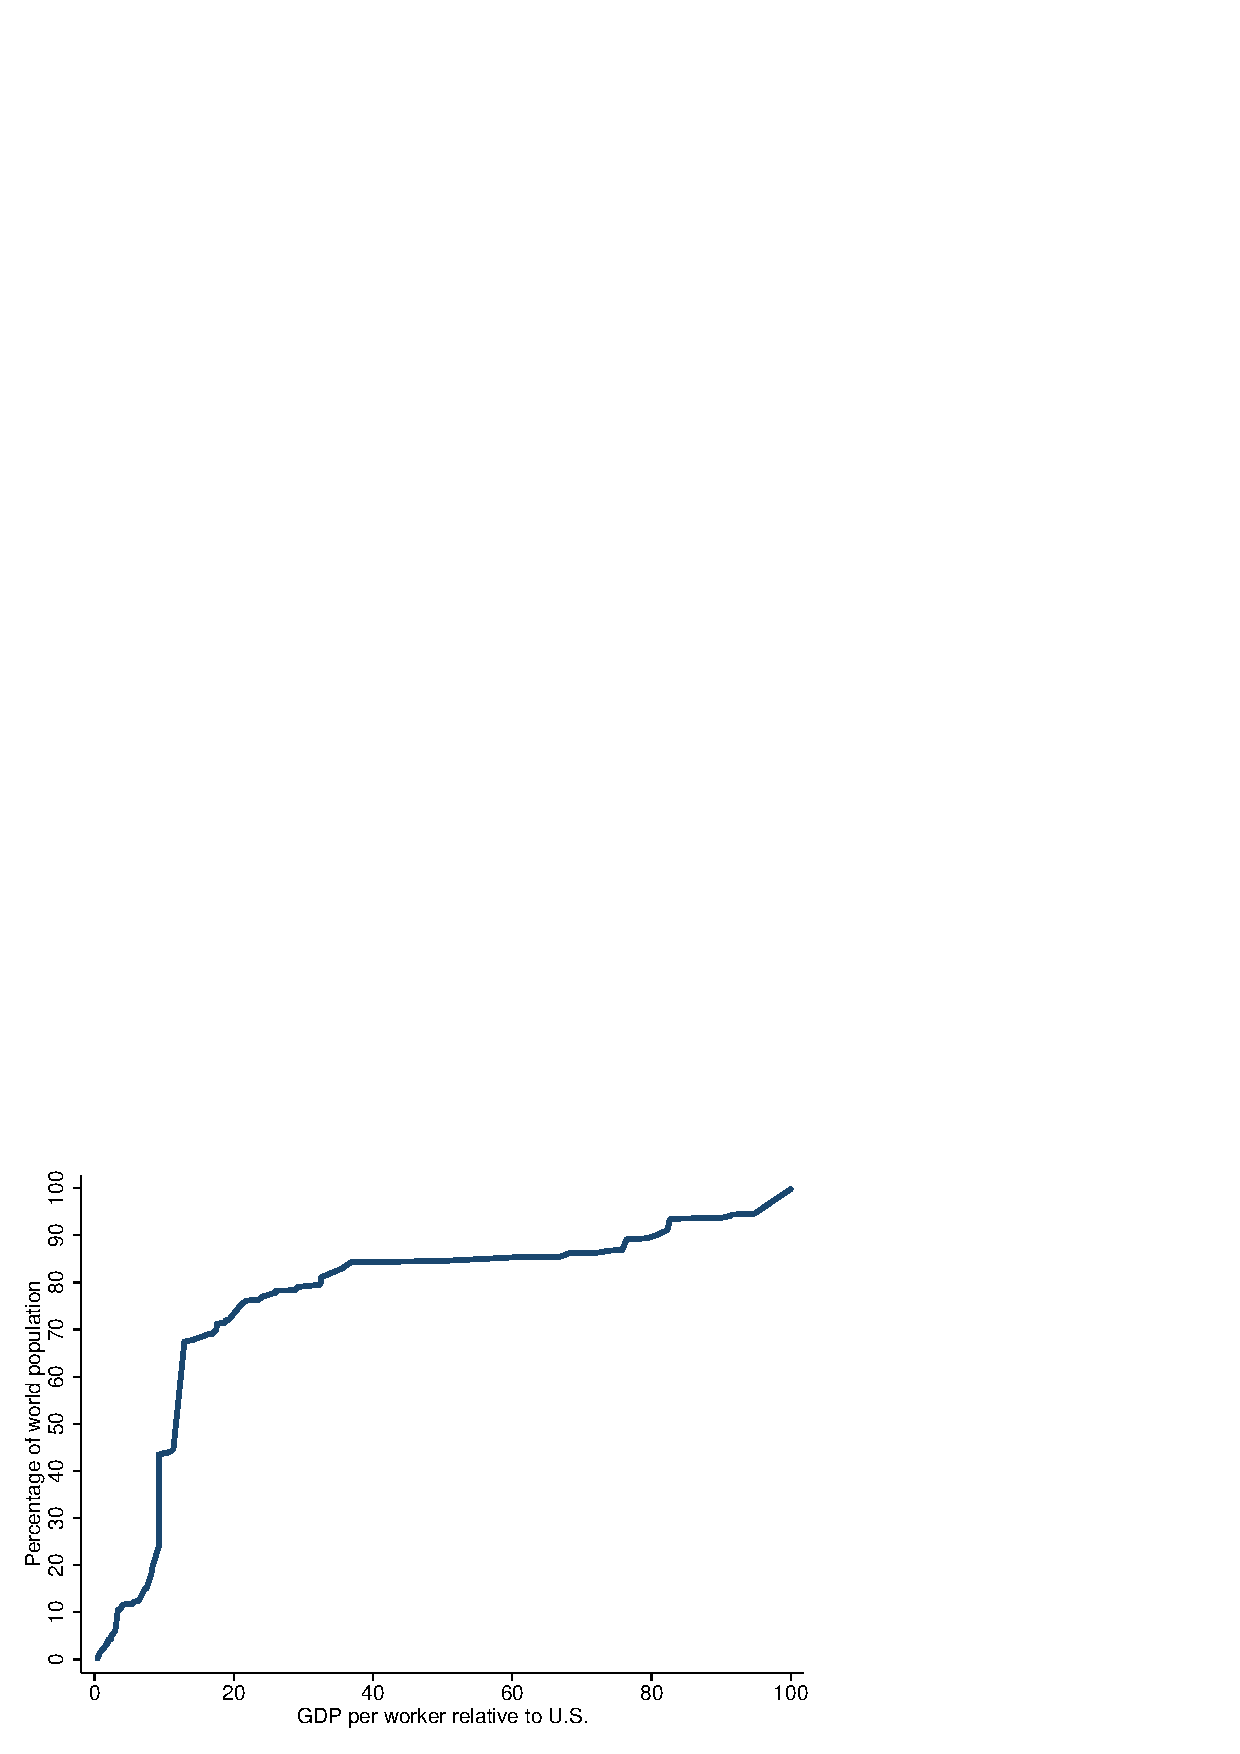
\includegraphics[scale=0.8]{graphs/figure_1_1.pdf}
\end{center}
\end{frame}

\begin{frame}
\frametitle{World Population by GDP per Worker, 1960 and 2008}
\begin{center}
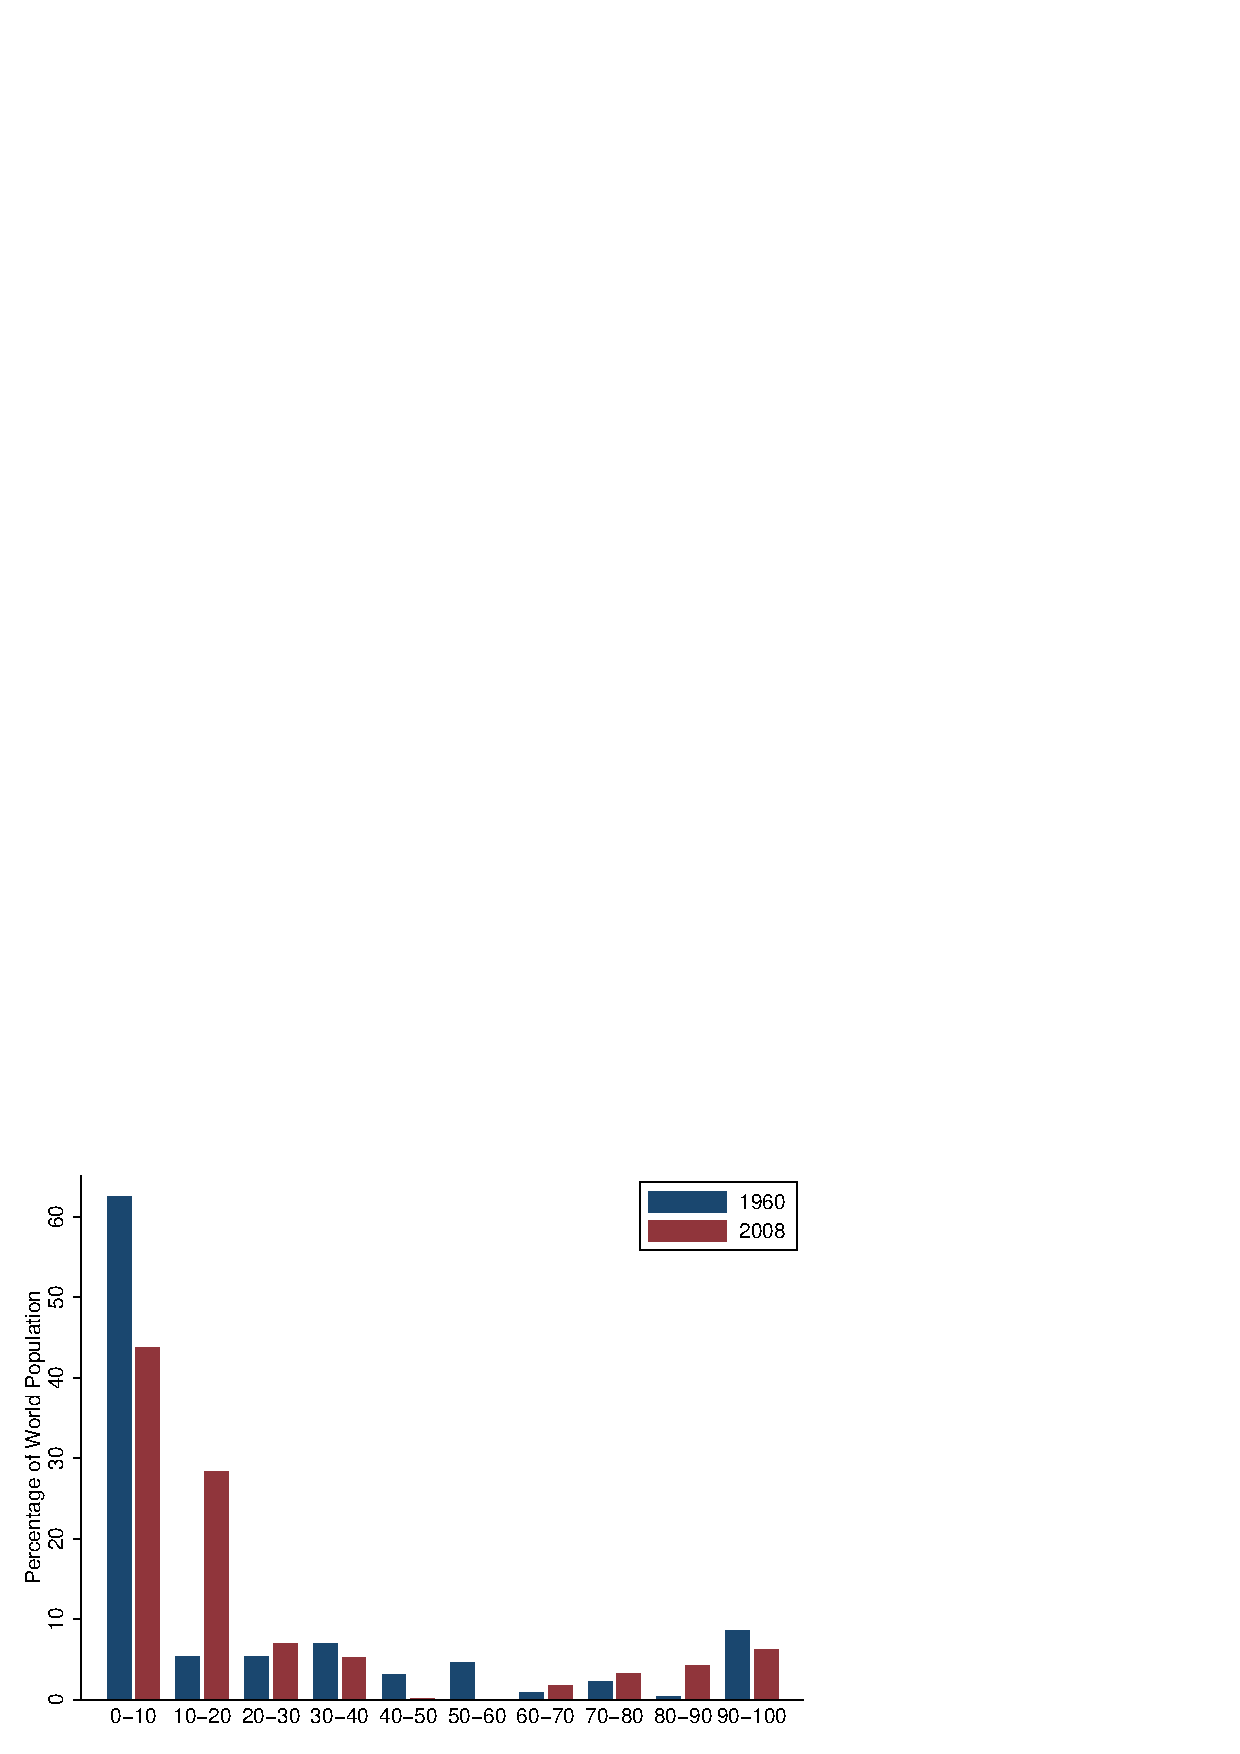
\includegraphics[scale=0.8]{graphs/figure_1_2.pdf}
\end{center}
\end{frame}

\begin{frame}
\frametitle{Introduction}
Fact 2: \textbf{Rates of economic growth vary substantially across countries.}

\vspace{.25in}\noindent Notes:
\begin{itemize}
	\item We will try to distinguish whether these are long-term differences or just transitional differences
	\item If they are long-term, then eventually some countries will be infinitely rich compared to others
	\item We think most differences are transitional
\end{itemize}
\end{frame}

\begin{frame}
Fact 3: \textbf{Growth rates are not generally constant over time. For the world as a whole, growth rates were close to zero over most of history but have increased sharply in the twentieth century. For individual countries, growth rates also change over time.}

\vspace{.25in}\noindent Note:
\begin{itemize}
	\item The big changes in growth rates over history are from pre-Industrial Revolution (close to 0\% growth) to modern times (roughly 1.85\% growth per year for developed countries)
	\item The big changes in growth rates within countries tend to be as they transition from poor to rich (e.g. Japan or China), after which growth slows down.
\end{itemize}
\end{frame}


\begin{frame}
\frametitle{World GDP per Capita Growth Rates}
\begin{center}
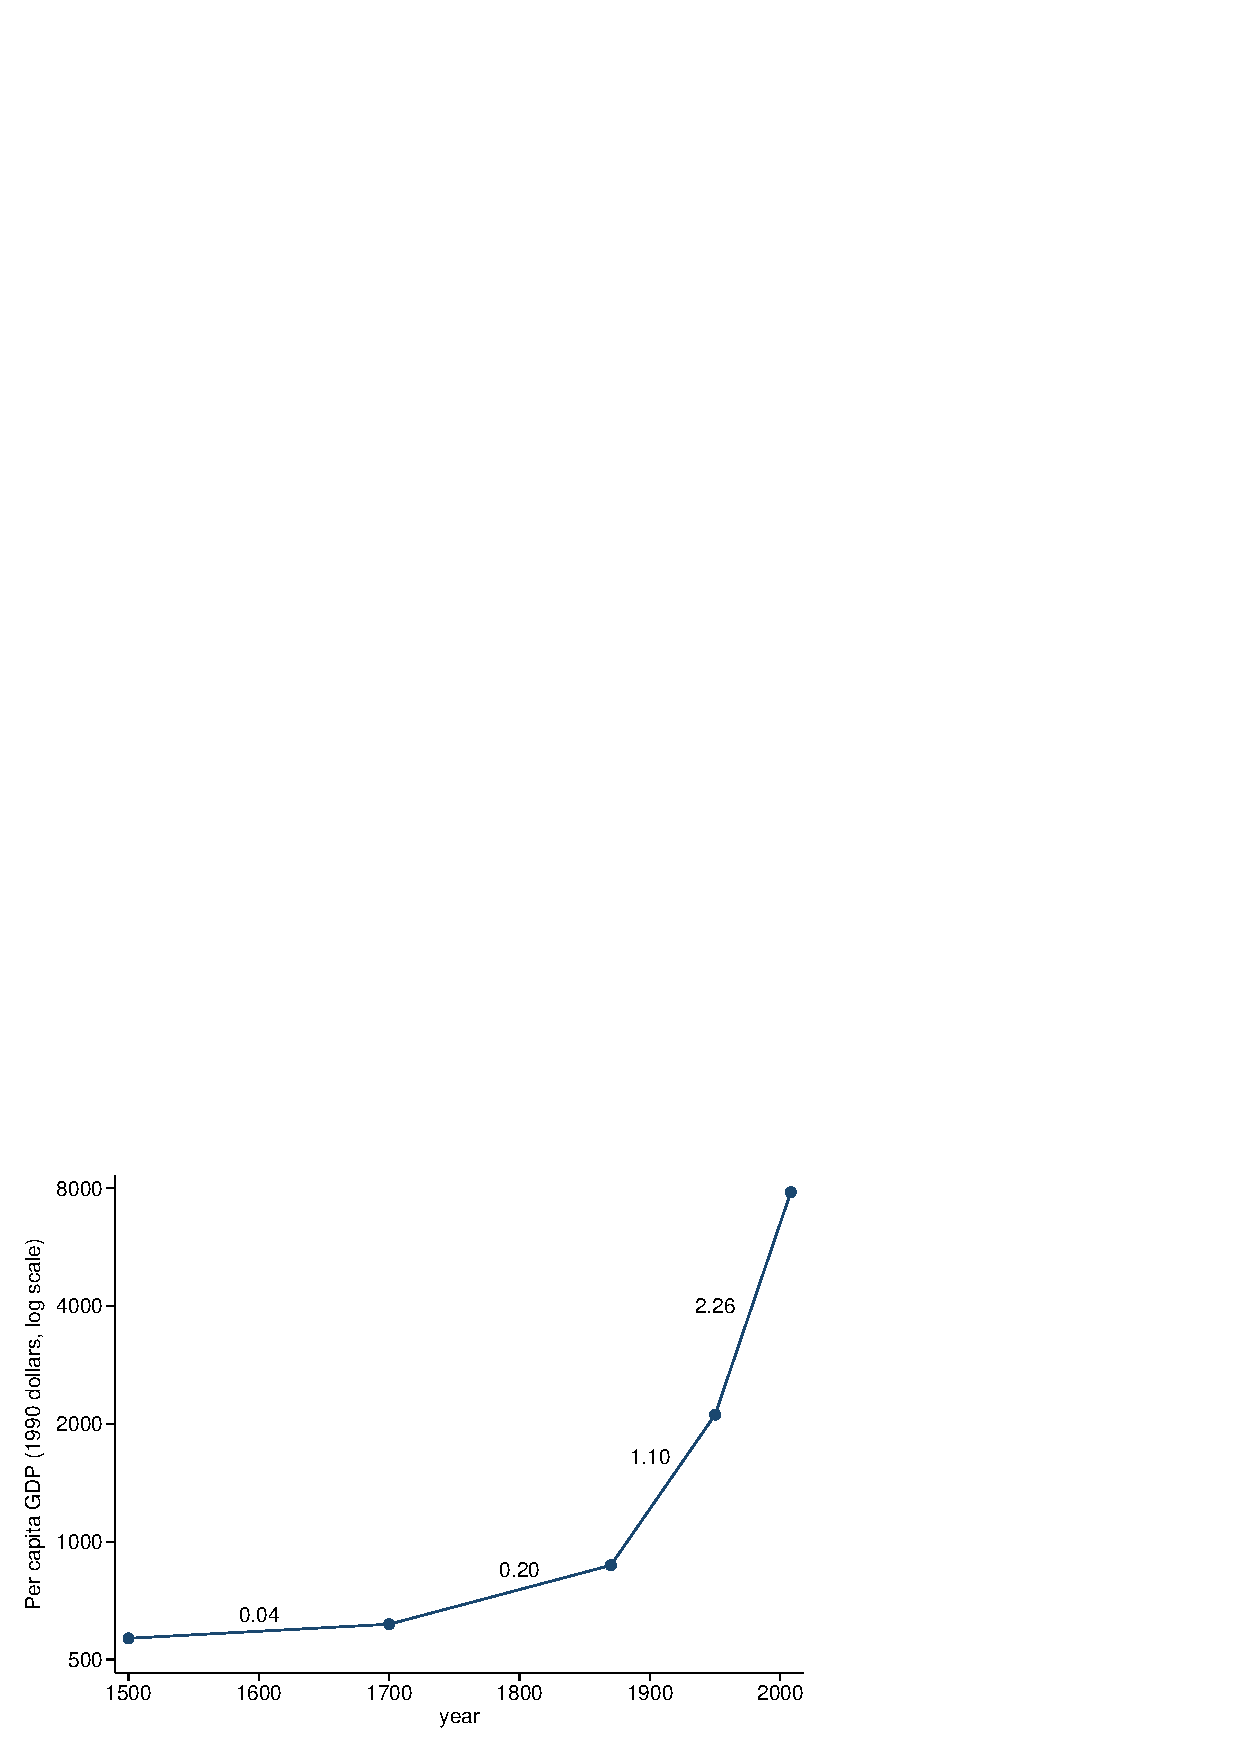
\includegraphics[scale=0.8]{graphs/figure_1_3.pdf}
\end{center}
\end{frame}


\begin{frame}
\frametitle{Introduction}
Fact 4: \textbf{A country's relative position in the world distribution of per capita incomes is not immutable. Countries can go from being ``poor'' to being ``rich'', and vice versa.}

\vspace{.25in}\noindent Notes:
\begin{itemize}
	\item The ``growth disasters'' in the table were all very well off in 1960 compared to East Asia. Now they are well behind
	\item The ``growth miracles'' in the table were though, in 1960, to be on the path to starvation and destitution. 
	\item What are the sources of these movements in rankings?
\end{itemize}
\end{frame}

\begin{frame}
Fact 5: \textbf{Growth in output and growth in the volume of international trade are closely related.}

\vspace{.25in}\noindent Notes:
\begin{itemize}
	\item Growth in trade is associated with growth in output, but not necessarily level of trade (Japan does not actually trade much, but is rich)
	\item Rapid growth in trade is no necessarily just growth in exports from East Asia (China and Korea also import a lot more than they used to)
\end{itemize}
\end{frame}

\begin{frame}
\frametitle{Growth in Trade and Growth in Output}
\begin{center}
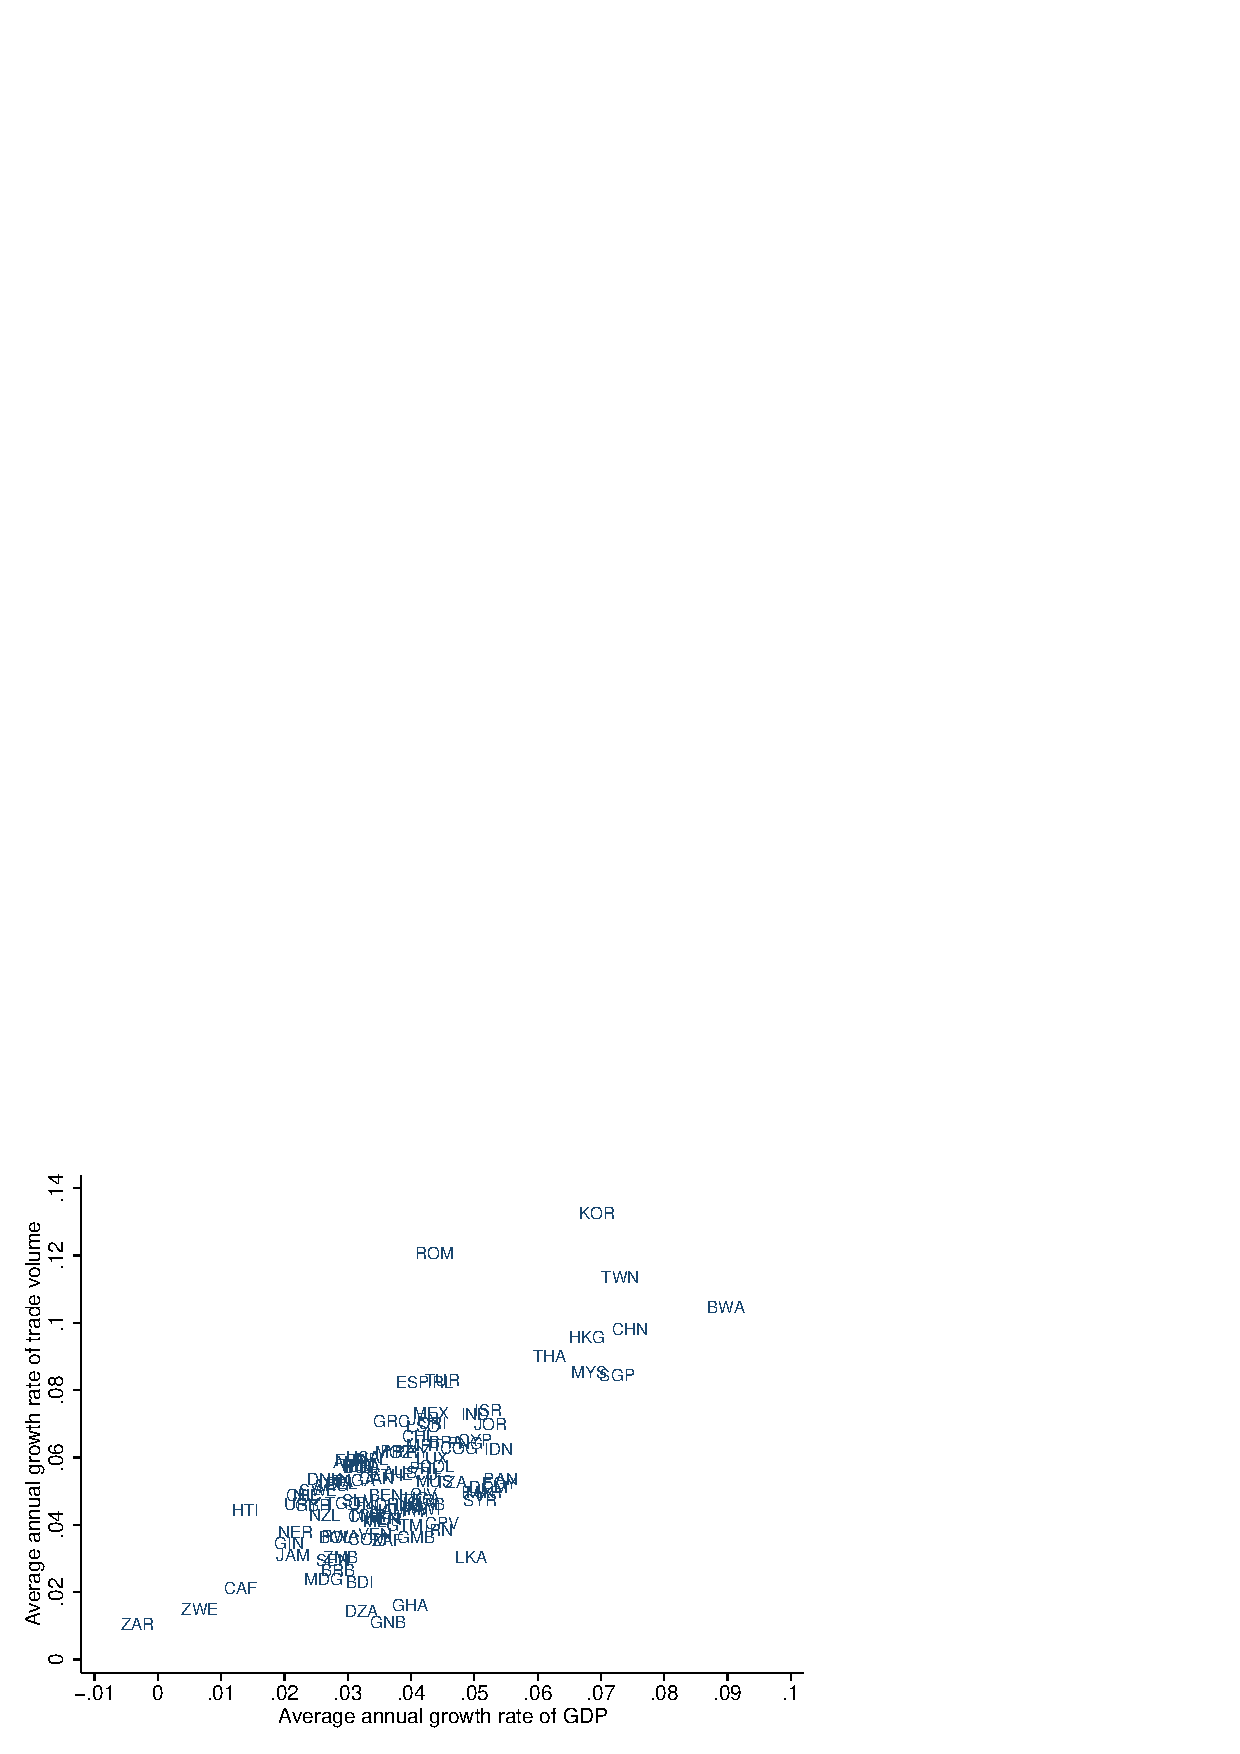
\includegraphics[scale=0.8]{graphs/figure_1_5.pdf}
\end{center}
\end{frame}


\begin{frame}
Fact 7: \textbf{Both skilled and unskilled workers tend to migrate from poor to rich countries or regions.}

\vspace{.25in}\noindent Notes:
\begin{itemize}
	\item Implies that return to both kinds of labour is higher in developed countries
	\item Shouldn't scarcity in poor countries imply a large premium to skilled workers?
\end{itemize}
\end{frame}


\begin{frame}
\frametitle{Big Questions}
\textbf{Why are some countries so rich and others so poor?}

\vspace{.25in}\noindent Answers?
\begin{itemize}
	\item Level differences
	\item Different levels of human capital
	\item Different institutions supporting innovation/technology adoption/entrepreneurship
\end{itemize}
\end{frame}


\begin{frame}
\frametitle{Big Questions}
\textbf{What is the engine of growth?}

\vspace{.25in}\noindent Answers?
\begin{itemize}
	\item Technological progress - new goods, or better versions of old goods
	\item Not accumulation of more physical or human capital - those cannot sustain growth
	\item Ultimately technological progress will rely on population - more people, more ideas
\end{itemize}
\end{frame}


\begin{frame}
\frametitle{Big Question}
\textbf{What creates growth miracles in some countries?}

\vspace{.25in}\noindent Answers?
\begin{itemize}
	\item Reversing what made them poor
	\item Changing institutions to foster technology adoption (copying?)
	\item Changing institutions to create larger markets (trade, internal markets) to support innovation/adoption
\end{itemize}
\end{frame}

\section{Standards of Living: Measurement}

\begin{frame}{PPP Measurement}
\textit{Assume that the average consumer in Russia and the average consumer in the United States buy the quantities and pay the prices indicated in the table below:} 
\\
    \begin{center}
    \begin{tabular}{lcccc}
       \hline 
        ~             & \multicolumn{2}{c}{Food}        & \multicolumn{2}{c}{Non-Food Item}       \\ \hline
        ~             & Price & Quantity & Price                   & Quantity \\ 
        Russia        & 300,000 Roubles     & 1      &  40,000 Roubles                    & 1      \\ 
        United States & \$10,000     & 1     & \$10,000                       & 1     \\ \hline
    \end{tabular}
    \end{center}
A few points:
\begin{itemize}
\item In Russia, an average person buys car once a 15 years.
\item \$1 = 10 Roubles.
\end{itemize}    
It turns out that per-capita consumption in Russia is \$2,000.
\end{frame}

\begin{frame}{PPP Measurement}
\begin{itemize}
\item We can improve upon the calculation we just did.
\item It would be nice if we have some common prices.
\item Let's say we use the American prices.
\item If we use American prices and substitute them into Russian bundle..\pause
\item .. Russian consumption is $0.07*100 + 1*10,000$
\item This type of computation is at the heart of PPP estimates.
\item These estimates use average prices across countries.
\end{itemize}
\end{frame}

\end{document}

